\documentclass[11pt, a4paper,twocolumn]{jarticle}
\usepackage[dvipdfmx]{graphicx}
\usepackage{listings,jlisting}

\begin{document}
%=============================================================
\section{二値周期パターンの取り込み}
\subsection{目的}
今回の実験は一次元方向にのみ光学濃度が変化する画像データの光信号の取得が目的である.

\subsection{手順}
まず図\ref{fig:8}に示す幅1.2mm,ピッチ2.4mmの二値周期パターン画像を光学系に取り付けた.
その後測定プログラムを実行し,データ点数1000,サンプリング周波数100Hzとして10秒間の測定を行った.

\begin{figure}[ht]
 \begin{center}
  
\includegraphics[width=0.8\linewidth]{fig8.png}
 \end{center}
 \caption{二値周期パターン}
 \label{fig:8}
\end{figure}

\subsection{結果}
測定の結果,図\ref{fig:9}のようになった.
周期的に変化する正弦波のような様子が測定できた.

\begin{figure}[ht]
 \begin{center}
  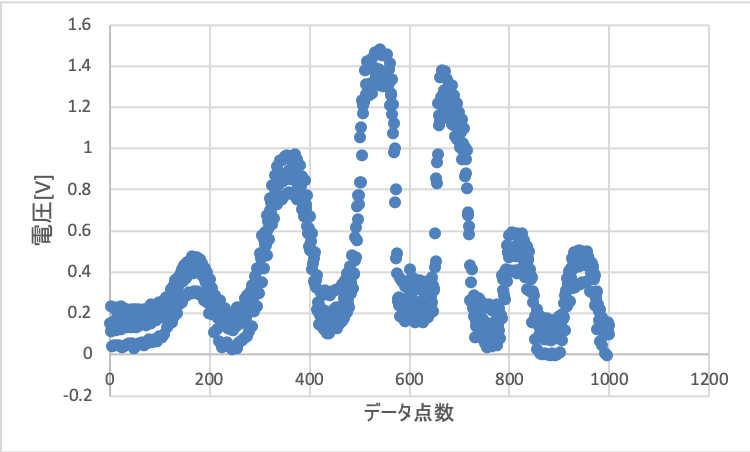
\includegraphics[width=0.8\linewidth]{fig9.png}
 \end{center}
 \caption{二値周期パターンの読み取り}
 \label{fig:9}
\end{figure}


\subsection{考察}
図\ref{fig:9}より4番目,5番目の周期が他の周期に比べて測定電圧が大きくなっているためこの時,コリメートされた光がレンズの中心を通り集光スポットが小さくなっていたと考えられる.
また実験5(ステッピングモーターの動作確認)で求めた1周期あたり$\Delta{x} = 0.0178mm$という値より,今回はエリアシングを起こすことなく正確に測定できたと考えられる.
測定結果がステップ関数のような二値ではなく滑らかな正弦波のようになった原因としては集光した光が入力物体に当たった際に散乱して周りの反射光も取り込んでしまったことや集光スポットが二値の境界線に乗ってしまったことなどが考えられる.
%=============================================================
\newpage
\end{document}
